\section{DBpedia}

\begin{frame}


\begin{minipage}{0.7\textwidth}
\begin{itemize}
  \item DBpedia gathers structured information from Wikipedia
	\begin{itemize}
	  \item infoboxes
	  \item tables, lists
	  \item images
	  \item categories
	  \item links
	  \item geocoordinates
	\end{itemize}
	\item
  \item english version currently describes 4 million things
  \begin{itemize}
    \item 832.000 persons, 639.000 places,
    372.000 creative works, 209.000 organizations, 226.000 species, 5.600
    diseases
    \end{itemize}
\end{itemize}
\end{minipage}
\hfill %wichtig, hier keine leerzeile im code
\begin{minipage}{0.25\textwidth}
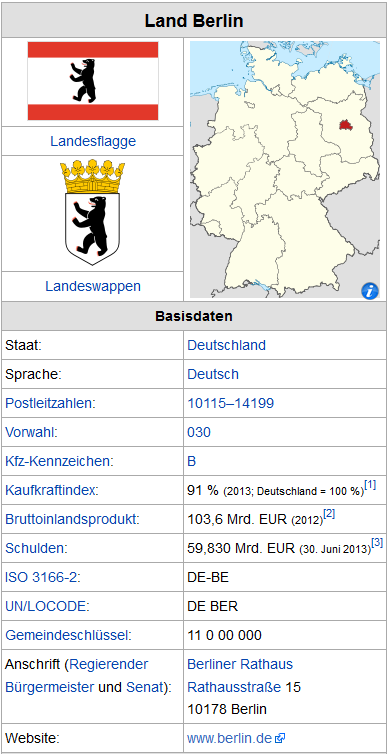
\includegraphics[scale=0.25]{img/berlin.png}
\end{minipage}
\end{frame}

\begin{frame}
\begin{itemize}
  \item 119 localized versions, in total:
  \begin{itemize}
    \item  12.6 million unique things
    \item 24.6 million links to images
    \item 27.6 million links to external web
    pages
    \item 45.0 million external links into other RDF datasets
    \item 67.0 million links to Wikipedia categories
    \item 41.2 million YAGO categories
  \end{itemize}
  \item
  \item Linked Data!
\end{itemize}
\end{frame}

\begin{frame}\centering
\begin{figure}
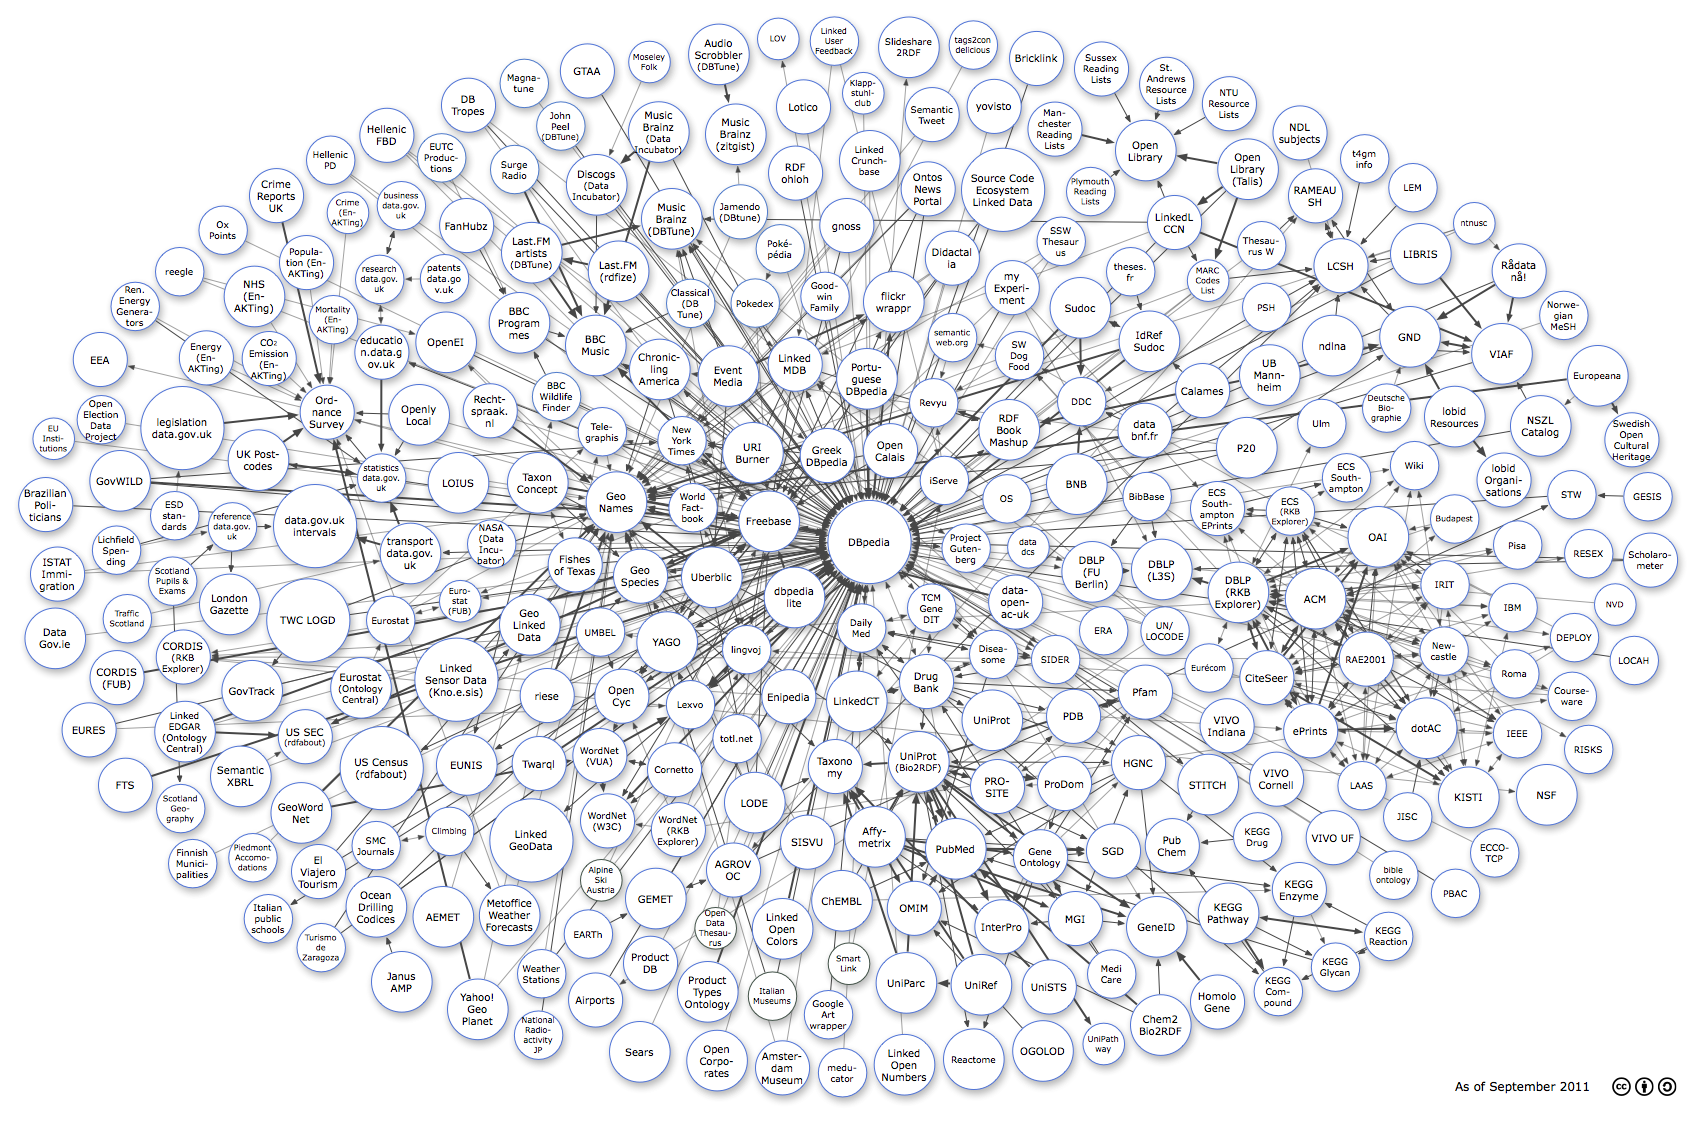
\includegraphics[scale=0.17]{img/lod-cloud.png}
\end{figure}
\small the web of data, by \url{http://lod-cloud.net/} (9/2011)
\end{frame}